\section{Introduction}
\label{sec:intro}
Predicting ``what happens next'' in narrative stories is an important
but challenging task of commonsense reasoning in artificial intelligence. 
Story comprehension was first studied in the context of 
planning and goal searching~\cite{meehan1977tale}, which was one of the
most important problems in AI. The task evolved~\cite{chambers2008unsupervised}
to predicting what is expected to happen next in stories. Much of the work
has been evaluated on a standard dataset called 
Story Cloze Test(SCT)~\cite{mostafazadeh2016corpus}. 
SCT asks for the correct ending of a four-sentence
story context from two alternatives, as shown in
\figref {fig:story}(a). 

\begin{figure}[th]
\centering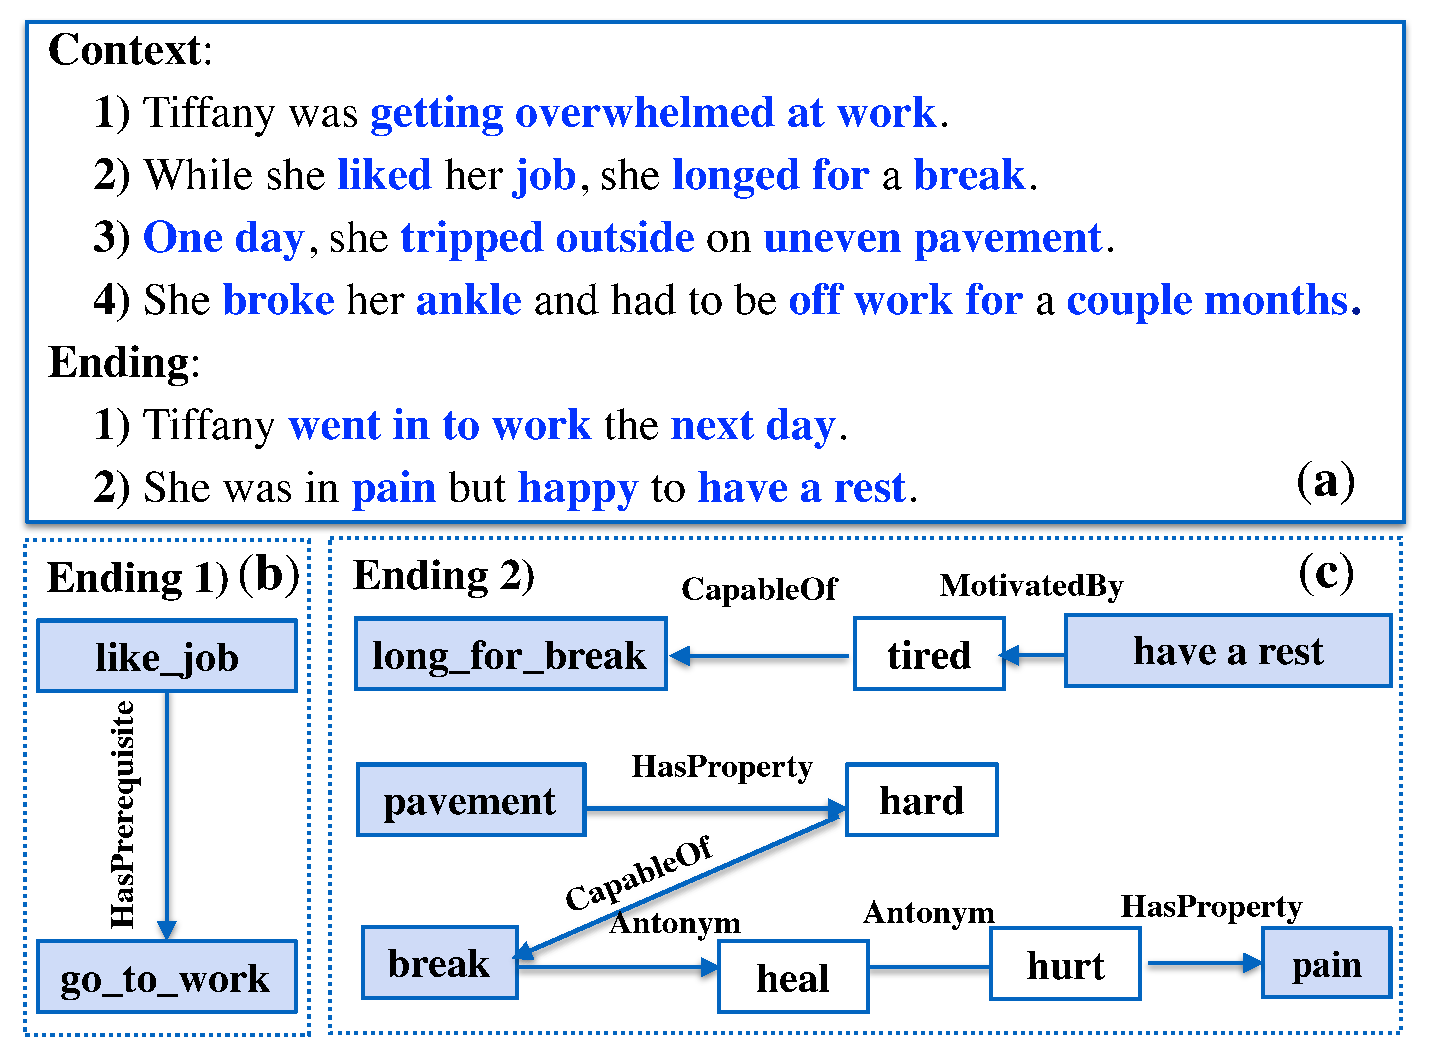
\includegraphics[width=3in]{pictures/story_example}
\caption{An example from the story-cloze task. 
In (b) and (c), the words in the blue boxes are concepts from the story; 
the words in the white boxes are concepts not from the story 
but serve as bridging nodes. }
%\KZ{Is it too early to talk about the concepts and briding nodes here? Maybe split this figure into two figs. Show (a) first, and then (b) and (c) later when you talk about the idea of solving SCT. (a) is only used to illustrate the problem. Also, in (a) instead of using ending (+) and ending (-), say possible ending 1 and possible ending 2. Whether it'scorrect or not is obvious to the reader.}}
%Ending (+) and ending (-) represent positive and negative ending for the context.}
\label{fig:story}
\end{figure}

%\begin{figure}[th]
%\small
%\begin{tabular}{ll} \hline
%\\
%Context: & Tiffany was \textcolor{blue}{getting overwhelmed at work}. \\
 %& While she \textcolor{blue}{liked} her \textcolor{blue}{job} she \textcolor{blue}{longed for} a \textcolor{blue}{break}. \\
 %& One day, she \textcolor{blue}{tripped outside} on uneven pavement. \\
 %& She \textcolor{blue}{broke} her \textcolor{blue}{ankle} and had to be \textcolor{blue}{off work} for \\
 %& a couple of months. \\
%Ending(+): & She was \textcolor{blue}{in pain} but \textcolor{blue}{happy} to \textcolor{blue}{not} have to \textcolor{blue}{go to work}. \\
%Ending(-): & She \textcolor{blue}{went in to work} the next day \\
%\\
 %\hline
%\end{tabular}
%\centering\includegraphics[width=3.5in]{pictures/story}
%\caption{Example from the story-cloze task: predict the correct ending to a given short story out of provided options.}\label{fig:story}
%\end{figure}

%We re-emphasize the deficiency of the over-reliance on information bias between 
%training and test data set that existed in many previous studies and 
%propose to apply a new way to compensate for this deficiency 
%in order to improve the authority of the assessment. 
%Most early studies treat this task as a supervised binary classification problem.
%However, this was not the original intention
%of \scite{mostafazadeh2016corpus} who proposed the SCT dataset, 
%because the training data has approximately 100,000 five-sentence stories,
%without any negative endings.
%%because the dataset didn't provide any
%%binary classification training data, but only approximately 100,000
%%five-sentence stories without negative endings.
%To overcome the lack of negative training data, 
%many researchers train their classifier using
%the smaller validation set from SCT, 
%which consists of 1,871 stories with annotated positive and negative endings.
%%the smaller validation set from SCT, which consists of both positive and
%In our study (\secref{sec:dataset}), we find there is significant bias in
%the positive and negative endings of the stories provided in the validation
%set, which causes information leak.
%We argue that human authorship of negative story endings is both unreliable and costly,
%and that validation set is not suitable for training
%or even fine-tuning the predicting models.
%%In addition, training with only about 1500 validation stories is contrary to ~\citeauthor{mostafazadeh2016corpus} 's original intention that actually understanding the underlying narrative from large quantity of narrative knowledge.
%%Instead, we propose to define the SCT story ending predicting task as a
%%semi-supervised learning problem. We train the prediction classifier on
%%the training set (with only positive endings),
%%as well as automatically generated negative endings.
%Instead, We propose to construct a new training set following ~\scite{roemmele2017rnn} 
%to reduce the correlation of training data and test data 
%on irrelevant features, so as to improve the reliability of the evaluation. 

Previous research on text inference mostly requires world knowledge
which is often extracted from large text corpus in the form of events and
organized into a structure. Such encoded knowledge is called scripts which has been used 
successfully on several narrative modeling tasks ~\cite{ferraro2016unified,orr2014learning,pichotta2016learning,peng2017joint}. 
%\KZ{Cite some more?}
Then at run time, the stories are also ``simplified'' into
a sequence of events, and inference is conducted using the knowledge structure and
the events in the stories.
%Scripts, is a type of encoding of worldly knowledge, and it have been used 
%successfully on several narrative 
%modeling tasks~. 
%Scripts was developed to represent stereotypical sequences of event 
%which is a unit of story featuring a world state change 
%\cite{prince1987dictionary}. 
The events (or frames in some of the work)
are mostly defined by analyzing the complex structure 
of the sentence through dependency parsing or semantic role labeling (SRL).
Because the definition of events in these approaches follows a 
strict linguistic theory and often rigid patterns, the extraction of
such events is a pipelined process and suffers from low accuracy and
low recall. For example, using 2-tuple event (verb, dependency)~\cite{ostermann2018mcscript}, 
we can only extract (break, Tiffany) and (be, Tiffany) from sentence 4) of \figref{fig:story}(a), missing out some
very important information for inference, such as ``ankle'', ``off work'' .
%However, The syntactic dependency events always utilize a very 
%impoverished representation of events in the specific form of elements, 
%for example two-tuple event (verb, dependency). 
%The role labeled events with long pipeline preprocessing will 
%result in an accumulation of errors and be over generalized.
%However, 
%the sparseness of data of events causes the information loss in the sentence
%representation. 

%Previous researches on this topic generally follow a two-step representation:
%first represent the individual sentence with shallow linguistic features,
%and then aggregate the sentence representations into a story context
%representation~\cite{mostafazadeh2016story,li2018multi,chen2018incorporating,zhou2019story}.
%Because most of these approaches use complex neural models
%with large number of parameters,
%they require large amount of training data.
%Unfortunately, stories for training come in limited quantity,
%and contain much variance and noises, distracting most of these models.
%Moreover, most of these methods did not properly model the
%commonsense relations between the sentences when aggregating
%the sentence representations.

%The first two genres represent the story from different perspectives.
%Many feature-based models represent a whole story with the external shallow
%linguistic features such as word embedding, character features,
%part-of-speech (POS) taggings, sentiment polarity of a word and
%negation~\cite{li2018multi}. However, these methods ignore the semantic
%structure in the story line, which is important for story understanding.
%The neural models represent each sentence with low-dimensional dense
%vectors~\cite{mostafazadeh2016story}.
%The sentence vectors are trained with different language models from
%a larger corpus, such as the BookCorpus, which contains 11,000 books.
%However, without sufficiently enough training resources, it is hard to
%learn the reasoning logic and an efficient representation.
%The third line incorporates the language features in neural model.
%For example, \citeauthor{chen2018incorporating} and ~\citeauthor{zhou2019story} apply
%ConceptNet~\cite{speer2017conceptnet}, a commonsence knowledge base,
%to extract the commonsense features between any two sentences in
%a story.

We propose a new text simplification method to remedy the above issues. 
We model sentences as a sequence of events and concepts, defined in
ConceptNet~\cite{speer2017conceptnet}, a community curated open-domain 
knowledge graph covering much of the knowledge required for commonsense 
reasoning.
The advantages of ConceptNet are i) events and concepts are defined
in the form of simple phrases, without complex structures, 
which makes matching at runtime easier; and ii) the relations
between the concepts are defined by humans and are presumed to be
more accurate.
In \figref{fig:story}(a), each colored phrase (multi-word expression) 
matches a concept from ConceptNet,
which is necessary ingredient for understanding the story.
Such event extraction is simple but nevertheless achieves 
decent performance without generalization or specific form. 
In this work, we improve the story representation
using commonsense knowledge from two aspects.
%\KZ{Move fig (b) and (c) here.}

First, we simplify each sentence by extracting a sequence of
ConceptNet concepts from the sentence
and obtain the {\em intra-sentence} concept representation.
%We keep only the concepts (colored words in \figref{fig:story}(a)
%from each sentence to represent the main idea of the story.
By simplifying the sentences, we essentially reduce the noise
and variance in the training data, which allows better performance
 given limited amount of data.
Then we use a sequential language model, inspired by
Skip-thought~\cite{kiros2015skip}, to obtain the
semantic representation of each simplified sentence. 
This encoding method has achieved good result on story ending 
reasoning task~\cite{roemmele2017rnn}. 
We will show for story ending prediction, this method is superior 
to GPT~\cite{radford2018improving} and BERT~\cite{devlin2018bert} pre-trained 
sentence encoding which has shown strong performance on many other 
NLP problems previously. 
%\KZ{But why not use GPT and other stronger language models? Shall we have a discussion here?}

Second, we incorporate structured commonsense knowledge 
from ConceptNet
%ConceptNet is first used on the story ending prediction task 
%by computing the concepts similarity between the ending and 
%context~\cite{chen2018incorporating}. For better use of 
by including the pre-trained concept 
embeddings in story sentence representation.  These embeddings encode
relations between the key concepts that exist in the contexts and the ending.
For example, in ~\figref{fig:story}(c),  ``long for break'' is related to ``have a rest''
through {\em CapableOf} and {\em MotivatedBy} relation edges.
These edges help us ``connect the dots'' within the story and allow us
to make more meaningful deduction through the story line.

In summary, this paper makes the following contributions:
%\KZ{Here depending on your contribution, you should make forward references to either approach section and eval sections.}
\begin{itemize}
\item We simplify the stories by streamlining sentences to a few
key concepts, which eliminates unwanted variance in the text (\secref{sec:sentence simplification}),
and achieve better results than
using the original sentences
% \KZ{How do you show that training is easier with the simplification of sentences in theevaluation?}
(\secref{sec:simplify});
\item We combine sequential and structured representation for the key concepts
in a sentence as the sentence representation~(\secref{sec:represent}) 
and show that such structured
knowledge is useful in understanding the stories
%This kind of representation takes into account the inter-sentence semantics
%and the external structured commonsense knowledge; 
(\secref{sec:ce});
\item Comprehensive experiments show that our story ending prediction
framework is effective in the end-to-end story cloze test and 
outperforms the other baselines by subtantial 
margains with valid training data(\secref{sec:result}).
\end{itemize}
